\section{Appendix}

\subsection{Additional ablation tables and figures}
\label{app:extra-figures}

\Cref{tab:app-blind-closure,tab:app-null-fix} give the full numbers for the candidate-blind closure
(\Cref{sec:analysis:deltaq}) and the rendered-null-line ablation (\Cref{sec:analysis:null}).
\Cref{fig:truncation} gives the long-state truncation histogram behind \Cref{sec:train:long}. The
serving-path engineering behind \Cref{sec:results:cost}, with \Cref{fig:serving}, is in
\Cref{app:serving}.

\begin{table}[h]
  \centering
  \caption{Candidate-blind $Z$, closure at full depth vs.\ the original tap-20 student.}
  \label{tab:app-blind-closure}
  \footnotesize
  \setlength{\tabcolsep}{4pt}
  \resizebox{\linewidth}{!}{%
  \begin{tabular}{lrrr}
    \toprule
    & Tap 20 & Full depth (28) & Teacher \\
    \midrule
    MMLU-Pro among-$K$ / choices-only / shuffled-q & .157 / .166 / .182 & .147 / .177 / .156 & .310 / .222 / .208 \\
    $\dq$ (choices-only) / $\dqsh$ (primary) & $-.009$ / $-.026$ & $-.030$ / $-.008$ & .088 / .102 \\
    SNLI / MNLI / ANLI / BoolQ & .905/.873/.541/.826 & .881/.807/.462/.712 & -- \\
    \bottomrule
  \end{tabular}}
\end{table}

\begin{table}[h]
  \centering
  \caption{Rendered $\nullsym$ line vs.\ the factored null, matched checkpoints (tap 20).}
  \label{tab:app-null-fix}
  \small
  \begin{tabular}{lrr}
    \toprule
    & Rendered $\nullsym$ line & Factored null (no rendered line) \\
    \midrule
    MMLU-Pro false-abstain rate & .692 & .003 \\
    MMLU-Pro accuracy & .133 & .353 \\
    Banking77 (unseen labels) accuracy / false-abstain & .063 / .924 & .579 / .135 \\
    CLINC-OOS accuracy / null AUROC & .639 / .840 & .798 / .973 \\
    $\dqsh$ (unchanged) & .118 & .122 \\
    \bottomrule
  \end{tabular}
\end{table}

\begin{figure}[h]
  \centering
  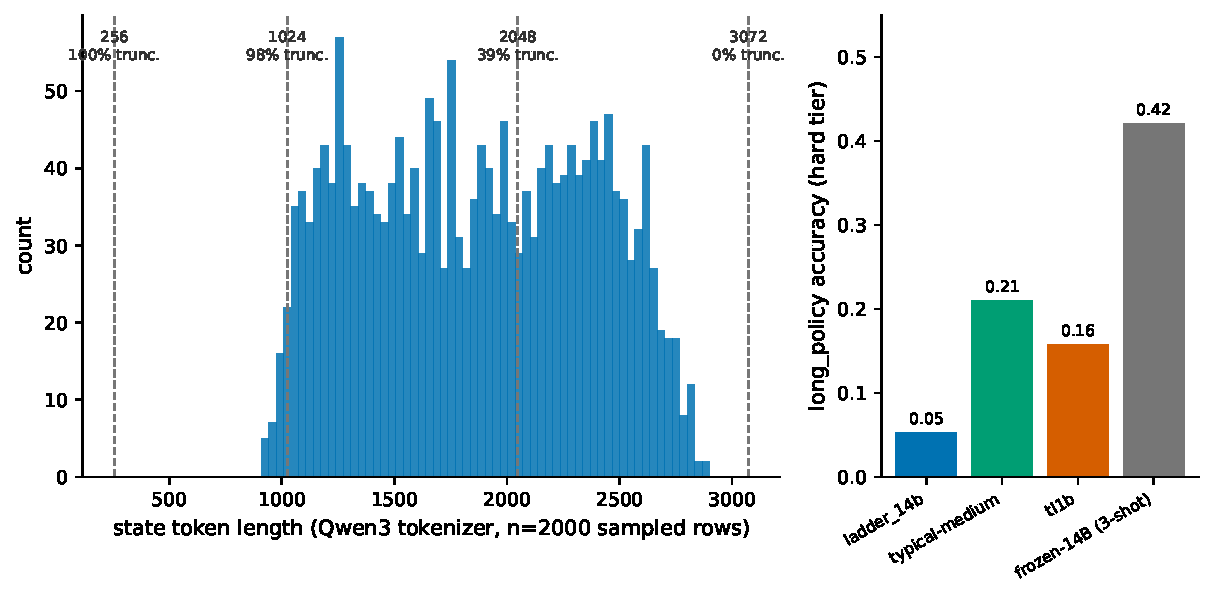
\includegraphics[width=\linewidth]{figures/fig_truncation.pdf}
  \caption{Left: histogram of \texttt{data\_wf\_long} state token lengths with truncation fractions at
  256/1024/2048/3072 tokens. Right: long\_policy (hard-tier) accuracy across the long-state bug/fix
  sequence.}
  \label{fig:truncation}
\end{figure}

\subsection{Native choice vs.\ energy scoring vs.\ batched log-probability, full $K$-sweep}
\label{app:latency-sweep}

\begin{figure}[h]
  \centering
  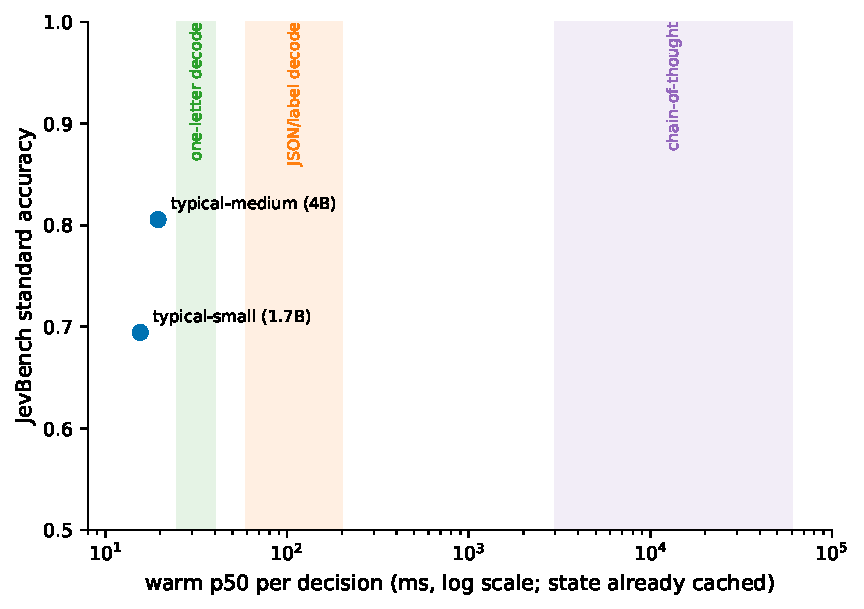
\includegraphics[width=\linewidth]{figures/fig_latency_quality.pdf}
  \caption{\textbf{Public subset, unranked.} JevBench standard accuracy vs.\ \emph{warm} per-decision
  p50 latency (ms, log scale) for the v1 release checkpoints (\texttt{ts1b}, \texttt{tm1b}), with
  generative-LLM decode-latency comparison bands. Latency is the served path with the state prefix
  already cached (\texttt{runs/serve\_bench2}, $\numcands{=}2$, 256-token state, one stream, in
  process, model load excluded), the same quantity as \Cref{app:serving}. The single-decision ladder of
  \Cref{tab:app-latency} measures a different quantity: it includes the state encode on the
  unoptimized path. Referenced from \Cref{sec:results:cost}.}
  \label{fig:latency_quality}
\end{figure}

At $M{=}256$ queries against one cached 256-token state, native choice's per-query marginal cost is
1.07, 1.55, 3.38, and 43.8\,ms at $K{=}2, 10, 32, 256$; a candidate-blind energy-scoring path is flat
at $\approx$1\,ms across the same range; and a baseline that re-runs the backbone once per candidate
costs 2.1, 4.6, 12.2, and 101.7\,ms. These values are transcribed from the run's log, because the
run's \texttt{bench.json} was lost to an out-of-memory crash. Batched marginal cost at $M{=}256$
scales more steeply with both size and $K$ than single-decision cost, from 2.7\,ms at 1.7B/$K{=}2$ to
110\,ms at 14B/$K{=}256$, so an energy-scoring front end gains value as the backbone grows.

\subsection{Serving-path engineering}
\label{app:serving}

The public inference package initially deep-copied the entire cached prefix's key-value tensors on every
decision. Replacing this with a zero-copy strided view plus cached attention masks and position tensors
reduced warm per-decision latency from 21--27\,ms to \textbf{15.5--17\,ms} (\texttt{typical-small} v1,
Qwen3-1.7B) and \textbf{19--21\,ms} (\texttt{typical-medium} v1, Qwen3-4B) on one H100
(\Cref{fig:serving}). \texttt{tm2} (Qwen3.5-4B, \texttt{typical-medium} v2) serves at 34--46\,ms warm
p50 on the same package with reference DeltaNet kernels. \texttt{torch.compile}/CUDA-graph capture
reached 8\,ms at a single fixed input shape, but probabilities shifted by up to .1 across the shape
buckets the serving path sees, and the mutable key-value cache produced stale-buffer crashes under the
standard capture-and-replay pattern, so we reverted it. Manual per-bucket graph capture is the remaining
path toward $\sim$10\,ms decisions.

\begin{figure}[h]
  \centering
  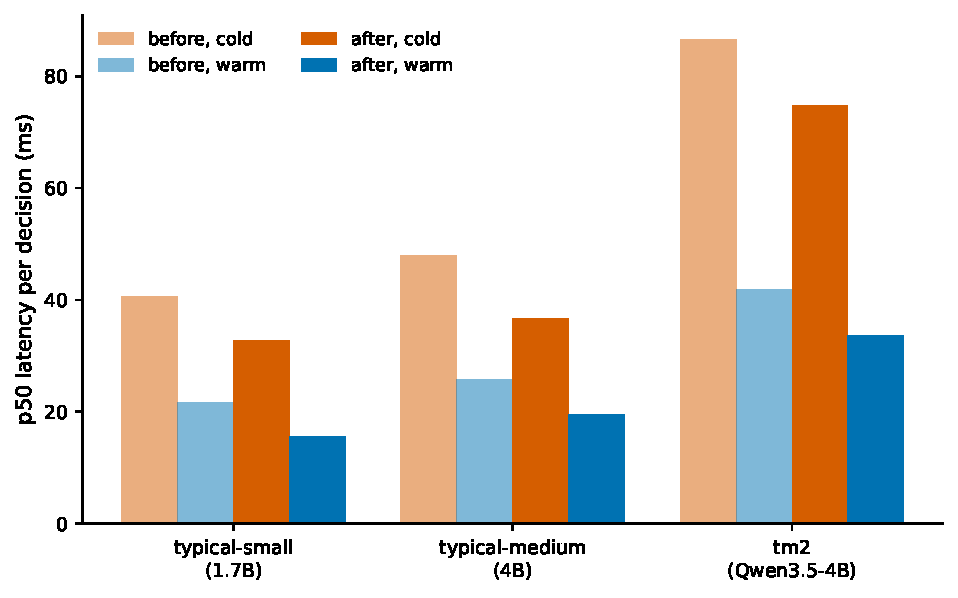
\includegraphics[width=\linewidth]{figures/fig_serving.pdf}
  \caption{Per-decision p50 latency before/after the zero-copy prefix fix, cold vs.\ warm, for
  \texttt{typical-small} v1 (1.7B), \texttt{typical-medium} v1 (Qwen3-4B), and \texttt{tm2}
  (Qwen3.5-4B, \texttt{typical-medium} v2), at $K{=}2$, 256-token state.}
  \label{fig:serving}
\end{figure}

\subsection{Mixture sweep, full table}
\label{app:mixture}

\begin{table}[h]
  \centering
  \caption{Mixture sweep at 1.7B, matched steps, referenced from \Cref{sec:results:mixture}. ``6A'' is the
  $E{:}0.35/K{:}0.25/W{:}0.40$ point; ``e45+null'' adds \texttt{null\_aug W:0.20} to
  $E{:}0.45/K{:}0.20/W{:}0.35$.}
  \label{tab:app-mixture}
  \small
  \setlength{\tabcolsep}{4pt}
  \begin{tabular}{lrrrrr}
    \toprule
    & Base ($E$ only) & 6A & e45 & \textbf{e45+null} & long$_{e45}$ (1024 tok) \\
    \midrule
    CLINC-150 acc / false-abstain & .845/.05 & .734/.17 & .779/.10 & \textbf{.805}/\textbf{.08} & .741/.13 \\
    MMLU-Pro among-$K$ / $\dqsh$ & .353/.122 & .330/.119 & .338/.115 & \textbf{.353}/\textbf{.143} & .329/.116 \\
    Held-out score NLL & -- & 2.03 & 1.52 & 2.04 & \textbf{1.26} \\
    JevBench std / hard & .694/.378 & .750/.387 & \textbf{.833}/.396 & .806/.396 & .806/\textbf{.450} \\
    \bottomrule
  \end{tabular}
\end{table}

Before the facts-first fix (\Cref{sec:train:long}), the long-state row (long$_{e45}$, 1{,}024 tokens,
25\% long-policy rows) alone raised \texttt{long\_policy} from .16 to .37 and \texttt{multi\_hop} from .17
to .28 relative to 6A, and gave the best soft-target NLLs of the sweep.

\subsection{Typed primitives: parameterization, routing, and full results}
\label{app:typed-primitives}

\textbf{Choice} is the $\numcands$-way readout of \Cref{sec:method:pass}, unchanged: a hard one-of-$K$
target trained with soft cross-entropy against \Cref{eq:factored-null}. \textbf{Score} is ordinal
(severity, quality, urgency). Plain Choice penalizes a one-level miss as much as an opposite-end miss, so
Score uses an ordinal-smoothed target,
\begin{equation}
  \label{eq:ordinal-smooth}
  \tilde{t}_j \propto \exp\!\left(-\frac{|j - y|}{\tauord}\right), \qquad \tauord = 0.7,
\end{equation}
normalized over valid levels, with $\tauord{=}0$ recovering one-hot Choice. This is a pure target change
with no architecture change. \textbf{Noul} is a yes/no proposition. Rendered as 2-way Choice it has no
order-invariance guarantee, since ``yes'' and ``no'' occupy two different suffix positions with two
different contextual states. Noul therefore gets a dedicated Bernoulli head that reads the query alone,
with no candidate text,
\begin{equation}
  \label{eq:bernoulli-noul}
  P(\text{yes}) = \sigma(w_n \cdot \hD),
\end{equation}
which is exactly order-invariant by construction and verified as an exact-zero reversed-label control.
The remaining mass $1{-}P(\text{yes})$ spreads over the other candidate(s), and the factored-null gate
still applies.

\textbf{Per-row routing.} A row is Noul-eligible iff its candidate set is exactly
$\{\text{yes},\text{no}\}$; every other row scores as ordinary Choice, bit-identical to a run with Noul
disabled. An early release candidate that applied the Bernoulli head at the \emph{model} level collapsed
to chance, because Choice- and Score-typed rows in the same batch were then scored with no candidate
text at all. Routing per row (verified by 140 unit tests) restored it. The type is a contract on the
input, and breaking that contract collapses accuracy to chance.

\begin{table}[h]
  \centering
  \caption{Typed primitives vs.\ their $K$-way Choice control, matched fine-tunes, referenced from
  \Cref{sec:results:typed}.}
  \label{tab:app-typed}
  \small
  \begin{tabular}{lrr}
    \toprule
    Score & $K$-way Choice & Ordinal-smoothed ($\tauord{=}0.7$) \\
    \midrule
    Held-out urgency: acc / NLL / ECE & .505 / 2.07 / .35 & .508 / \textbf{1.23} / \textbf{.19} \\
    JevBench hard: acc / Brier & .360 / .88 & \textbf{.459} / \textbf{.70} \\
    JevBench ordinal items (12), decisions changed & -- & 0 of 12 \\
    \midrule
    Noul & 2-way Choice & Bernoulli \\
    \midrule
    PagerDuty (floor .792): acc / NLL & .602 / 1.04 & \textbf{.886} / \textbf{.28} \\
    Reversed-label max $|\Delta P(\mathrm{yes})|$ & .55 & \textbf{0} (exact, all sets) \\
    \bottomrule
  \end{tabular}
\end{table}

\subsection{DecisionMix v2, full numbers}
\label{app:decisionmix}

Held-out family/grammar/style accuracy moves from .48/.51/.49 (matched control, never trained on
\texttt{data\_wh}) to .83/.88/.89 (DecisionMix v2), and rubric-flip accuracy moves from .48 to .71,
measured within the generator's own rule engine (\Cref{sec:train:rubric}). The uncertainty corpus moves
typed-decisions NLL from 2.06 to 1.71 (\Cref{sec:train:uncertainty}). Level-7 composition is in
\Cref{app:hard-tier}.

\subsection{Full hyperparameters}
\label{app:hyperparams}

\Cref{tab:app-hparams} gives the exact configuration of each checkpoint in the paper. All runs use AdamW,
bf16, and LoRA rank 16 on the top eight kept layers of the truncated backbone; the family-balanced sampler
and null augmentation are described in \Cref{sec:train:mixture,sec:train:nullaug}.

\begin{table}[h]
  \centering
  \caption{Training configuration by checkpoint. Tap is given as layer / total layers of the base model.
  $E{:}K{:}W{:}U$ is the family-sampler weight per batch. Max state is the training-time token budget for
  the cached prefix.}
  \label{tab:app-hparams}
  \footnotesize
  \setlength{\tabcolsep}{3pt}
  \resizebox{\linewidth}{!}{%
  \begin{tabular}{lrrrrrr}
    \toprule
    Checkpoint & Backbone & Tap & Steps & Batch & $E{:}K{:}W{:}U$ & Max state \\
    \midrule
    \texttt{typical-small-preview} & Qwen3-1.7B-Base & 20/28 & 12{,}000 & 64 & .35{:}.25{:}.40{:}0 & 256 \\
    \texttt{ts1b} (\texttt{typical-small} v1) & Qwen3-1.7B-Base & 20/28 & 12{,}000 & 64 & .40{:}.15{:}.35{:}.10 & 1{,}024 \\
    \texttt{tm1b} (\texttt{typical-medium} v1) & Qwen3-4B-Base & 26/36 & 12{,}000 & 64 & .40{:}.15{:}.35{:}.10 & 1{,}024 \\
    \texttt{ladder\_8b} & Qwen3-8B-Base & 26/36 & 12{,}000 & 64 & .35{:}.25{:}.40{:}0 & 256 \\
    \texttt{ladder\_14b} & Qwen3-14B-Base & 28/40 & 12{,}000 & 64 & .35{:}.25{:}.40{:}0 & 256 \\
    \texttt{tl1b} (14B) & Qwen3-14B-Base & 28/40 & 8{,}000 & 64 & DecisionMix v2 + $U$, facts-first & 3{,}072 \\
    \texttt{tm2} (\texttt{typical-medium} v2) & Qwen3.5-4B-Base & $\approx$71\% & 12{,}000 & 64 & .40{:}.15{:}.35{:}.10 & 2{,}048 \\
    \bottomrule
  \end{tabular}}
\end{table}

\texttt{ts1b}/\texttt{tm1b} additionally set \texttt{null\_aug W:0.20}, \texttt{ordinal\_smooth 0.7} (Score),
\texttt{noul\_head bern} (routed per row, \Cref{sec:method:typed}), \texttt{null factored}, and
\texttt{nc\_render letters\_nonull}. \texttt{tl1b} adds \texttt{--drop\_truncated}, frozen-teacher KD
($\alpha \cdot \mathrm{CE} + \beta \cdot \mathrm{KL}$, $T{=}2$, against the same backbone's own frozen
3-shot letter distribution on 63k labelled rows), and checkpoint selection on held-out
uncertainty-plus-curriculum validation NLL (\texttt{--best\_on}) in place of in-distribution loss. Final
fitted temperature and null offset for \texttt{ts1b}: $T{=}1.124$, offset $0$ (post-hoc, applied at eval).
\texttt{ts1c} (\texttt{typical-small} v2) is the 1.7B model trained on the facts-first long-state corpus;
its long-state and JevBench numbers are in \Cref{tab:app-long-release}.

\subsection{Corpus construction detail}
\label{app:corpora}

\textbf{\texttt{data\_v5}} (633{,}213 train / 4{,}001 val rows) covers evidence tasks and classification
with a deliberately wide span of label vocabularies at low rows-per-source, so the model cannot memorize a
fixed small set of label sets and must read the rendered options. \textbf{\texttt{data\_kb}} (147{,}447
train / 3{,}001 val) is distilled from ARC-Easy/Challenge, OpenBookQA, CommonsenseQA, SciQ, QASC, LogiQA,
AQuA-RAT, MedMCQA, and MMLU-auxiliary-train, with TruthfulQA-MC1 held out entirely and two items excluded
from all MMLU-Pro numbers after a leakage audit against that evaluation set. \textbf{\texttt{data\_wf}}
(72{,}006 train / 3{,}000 val) is our own rubric-conditioned workflow generator, 15 families of
Noul/Choice/Score decisions (policy checks, adequacy, support, fact verification, eligibility, routing,
action selection, enumeration extraction, categorical judgment, tool selection, and four ordinal
quality/severity/relevance/completeness scales, plus urgency); three whole families (eligibility,
tool\_select, urgency, one per type) are held out of training entirely, and 26{,}513 of the 72{,}006 rows
belong to \emph{rubric groups}: the same state and candidate set rendered under two or three different
rubrics with different gold answers, built to measure and train rubric dependence over
state/candidate pattern-matching. \textbf{\texttt{data\_wf\_hf}} (86{,}600 train rows) adds three
externally sourced sets in the same typed shape: \texttt{cua-s1-forms} (60{,}000 rows, procedural GUI-form
option-scoring, MIT license, with a form-signature-disjoint 24{,}370-row test split and a 196-row
real-usage demo split held out), \texttt{systemone-lite-general} (20{,}000 rows, rule-labeled typed
decisions, MIT, with a 5{,}400-row hard split held out), and \texttt{jev-4b-distill-data} (6{,}600 rows,
programmatic gold, Apache-2.0, with a 600-row adversarial split held out). \textbf{\texttt{data\_wf\_long}}
(23{,}318 train rows) is a longer-state variant of the workflow generator for multi-paragraph policy
documents, rendered facts-first (\Cref{sec:train:long}). \textbf{\texttt{data\_wh}} (60{,}605 train /
3{,}000 val) is a second, independent rubric-conditioned generator (DecisionMix v2): a programmatic rule
engine over 12 domains and six boolean conditions at seven levels of compositional depth, where levels
1--6 are trained and level 7 (compositions requiring temporal, unit-conversion, expected-value, or
trade-off reasoning that the generator does not otherwise produce) is evaluation-only; every trained row
belongs to a counterfactual rubric group. One whole domain/level pair, three whole domains, and two rubric
styles are held out. \textbf{\texttt{data\_u}} (31{,}029 train / 2{,}000 val) is a soft-target uncertainty
corpus: the validation split of UNLI, the ambiguous rows of AmbiEnt (uniform target over the listed
labels), and four synthetic generators with exact closed-form posteriors (partial-evidence combination, a
noisy-sensor Bayesian update, ordinal confusion via an inverted confusion matrix, and conflicting-sources
log-odds pooling), each with a held-out parameter range; ChaosNLI-ambiguity (MNLI portion) is
evaluation-only.

\begin{table}[h]
  \centering
  \caption{\texttt{data\_wf}: 15 families, 72{,}006 train rows, 3 held out (marked *). ``In rubric groups''
  counts rows that are part of a same-state-same-candidates, different-rubric-different-gold group.}
  \label{tab:app-wf}
  \small
  \begin{tabular}{llrr}
    \toprule
    Family & Type & Rows & In rubric groups \\
    \midrule
    policy\_permit & Noul & 9{,}000 & 5{,}205 \\
    adequacy & Noul & 5{,}000 & 0 \\
    support & Noul & 6{,}000 & 0 \\
    fact & Noul & 5{,}000 & 0 \\
    eligibility* & Noul & 1{,}500 & 851 \\
    routing & Choice & 9{,}003 & 5{,}208 \\
    action\_select & Choice & 7{,}000 & 4{,}054 \\
    enum\_extract & Choice & 7{,}000 & 3{,}618 \\
    categorical & Choice & 7{,}004 & 3{,}882 \\
    tool\_select* & Choice & 1{,}500 & 905 \\
    quality & Score & 6{,}000 & 0 \\
    severity & Score & 6{,}000 & 3{,}497 \\
    relevance & Score & 3{,}998 & 0 \\
    completeness & Score & 4{,}001 & 2{,}196 \\
    urgency* & Score & 1{,}502 & 900 \\
    \bottomrule
  \end{tabular}
\end{table}

\begin{table}[h]
  \centering
  \caption{\texttt{data\_wh} (DecisionMix v2): 60{,}605 train rows across 12 domains $\times$ 6 boolean
  conditions, levels 1--6; level 7 (temporal/numeric/probability/trade-off composition) is eval-only.}
  \label{tab:app-wh}
  \small
  \begin{tabular}{lrr}
    \toprule
    Level & Train rows & Held-out grammar rows \\
    \midrule
    1 & 10{,}601 & 142 \\
    2 & 10{,}600 & 141 \\
    3 & 10{,}600 & 141 \\
    4 & 10{,}601 & 140 \\
    5 & 10{,}602 & 142 \\
    6 & 10{,}601 & 141 \\
    \bottomrule
  \end{tabular}
  \quad
  \begin{tabular}{lr}
    \toprule
    Eval file & Rows \\
    \midrule
    \texttt{wh\_heldout\_family} & 422 \\
    \texttt{wh\_heldout\_style} & 403 \\
    \texttt{wh\_heldout\_grammar} & 816 \\
    \texttt{wh\_level7} & 880 \\
    \texttt{wh\_rubric\_flip} & 2{,}206 \\
    \texttt{wh\_rubric\_shuffled} & 2{,}437 \\
    \bottomrule
  \end{tabular}
\end{table}

\begin{table}[h]
  \centering
  \caption{\texttt{data\_u}: 31{,}029 train rows, 100\% soft-target.}
  \label{tab:app-u}
  \small
  \begin{tabular}{lr}
    \toprule
    Source & Train rows \\
    \midrule
    Synthetic (4 closed-form generators) & 28{,}560 \\
    UNLI (validation split only) & 2{,}068 \\
    AmbiEnt (ambiguous rows) & 401 \\
    \midrule
    By decision type: Noul / Score / Choice & 23{,}403 / 7{,}225 / 401 \\
    \bottomrule
  \end{tabular}
\end{table}

\subsection{Hard compositional tier and the frozen 14B comparison}
\label{app:hard-tier}

Compositions deeper than anything in training are the frontier of single-pass readout, and this
subsection collects the measurements that locate it. Rubric-conditioned training moves held-out
families, grammars and styles inside the generator's distribution to .84--.90
(\Cref{app:decisionmix}). Level-7 composition, which requires temporal arithmetic, unit conversion,
expected-value reasoning or multi-attribute trade-offs, moves far less. On the 880-item level-7 set the
uniform-guess rate is .441 (598 items at $\numcands{=}2$, 224 at 3, 58 at 4; the majority-class rate is
.250), and the checkpoints score .493 (\texttt{ts1b}), .544 (\texttt{tm1b}) and .620 (\texttt{tl1b}).
The 14B checkpoint is the one clearly above the guess rate, and all three sit 25--40 points below their
own in-distribution held-out scores: the curriculum that moves every in-distribution family by more than
30 points moves level 7 by 5. The JevBench hard tier's temporal, probability and trade-off families
show the same pattern.

\begin{table}[h]
  \centering
  \caption{14B comparisons. \textbf{JevBench: public 231-id subset, unranked}; 95\% cluster-bootstrap
  intervals over the paraphrase \texttt{group} field ($n_{\mathrm{eff}}{=}36$ standard states,
  $n{=}111$ hard items). \texttt{tl1b\_nokd} is identical to \texttt{tl1b} in every flag except
  \texttt{--distill\_beta 0}. Paired per-item tests are in the text; the marginal intervals overlap and
  are not the basis for any comparison.}
  \label{tab:tl1b}
  \small
  \setlength{\tabcolsep}{2pt}
  \begin{tabular}{lcccc}
    \toprule
    & \texttt{ladder\_14b} & \texttt{tl1b} & \texttt{tl1b\_nokd} & Frozen, 3-shot \\
    \midrule
    JevBench std & .875 [.792, .944] & .931 [.861, .986] & .917 [.833, .986] & .819 [.708, .917] \\
    JevBench hard & .468 [.378, .559] & .450 [.360, .541] & .477 [.387, .568] & \textbf{.559} [.468, .649] \\
    JevBench Brier std (hard) & .173 (.85) & .175 (.66) & .127 (--) & .30 (.60) \\
    \texttt{long\_policy} (hard subfamily) & .053 & .158 & .211 & \textbf{.421} \\
    Training val NLL & -- & .438 & .410 & -- \\
    Held-out score NLL & 2.87 & \textbf{0.95} & -- & -- \\
    Level-7 composition (guess rate .441) & -- & .620 & -- & -- \\
    \bottomrule
  \end{tabular}
\end{table}

\textbf{The frozen 14B backbone with three exemplars leads the trained 14B on the hard tier.}
\Cref{tab:tl1b} compares the previous-recipe 14B checkpoint (\texttt{ladder\_14b}); the bundle that
fixed the long-state rendering, dropped over-length rows, and added DecisionMix v2, the typed heads and
calibration-shaped checkpoint selection (\texttt{tl1b}); the same bundle without frozen-teacher
distillation (\texttt{tl1b\_nokd}); and the frozen backbone with three exemplars. A paired cluster
bootstrap on the per-item difference over the same 111 hard items gives frozen-minus-trained $+.108$
$[+.027, +.189]$, $p{=}.015$ against \texttt{tl1b}, and $+.081$ $[-.009, +.171]$, $p{=}.082$ against
\texttt{tl1b\_nokd}. On the standard tier the ordering reverses (frozen-minus-trained $-.111$
$[-.250, +.014]$, $p{=}.10$). The frozen control is scored with a 3-shot letter-logit rendering that
was not swept; rendering alone moves a frozen 9B checkpoint by 12.5 standard-tier points
(\Cref{tab:rendering}).

\textbf{The backbone carries hard-tier behavior that the current recipe does not preserve.} Per family
(\Cref{fig:hard_families}, \Cref{tab:app-hard}), the frozen 14B leads \texttt{tl1b} on
\texttt{tradeoff} (.500 vs.\ .167), \texttt{long\_policy} (.421 vs.\ .158), \texttt{ambiguous} (.714
vs.\ .429), \texttt{probability} (.500 vs.\ .300) and \texttt{temporal\_numeric} (.333 vs.\ .200), and
trails on \texttt{multi\_hop} (.444 vs.\ .611). Families hold 3--19 items and no single family
separates; the direction is the same across every serial family. Our generators compose boolean rules up
to six levels deep and never produce the temporal, probability and trade-off operations these families
use, which explains why training did not add the behavior. The measurement that separates missing
coverage from a limit of fixed-depth computation is the same frozen backbone given a scratchpad on the
same 111 items; \Cref{sec:discussion} takes this up.

\textbf{Same-backbone frozen-teacher distillation has no detectable effect.} It is the one component of
the 14B bundle with its own matched control. \texttt{tl1b\_nokd} is nominally ahead on hard accuracy
(.477 vs.\ .450), \texttt{long\_policy} (.211 vs.\ .158), training validation NLL (.410 vs.\ .438) and
standard-tier Brier (.127 vs.\ .175), and \texttt{tl1b} is nominally ahead on standard accuracy (.931
vs.\ .917). The paired bootstraps are $-.027$ $[-.090, +.027]$ ($p{=}.45$) on hard and $+.014$
$[-.042, +.069]$ ($p{=}.81$) on standard.

\textbf{The bundle's clear effect is on probability quality.} The \texttt{ladder\_14b} $\to$
\texttt{tl1b} standard-tier change is .875 $\to$ .931 (paired $+.056$ $[+.000, +.125]$, $p{=}.13$).
Held-out score NLL falls from 2.87 to 0.95 and hard-tier Brier from .85 to .66, both large relative to
their noise.

\textbf{The same question on 19 JevBench items.} \texttt{ladder\_14b} scores .053 on the JevBench
\texttt{long\_policy} family ($n{=}19$) and .919 on the 605 held-out long states in its own training
render (\Cref{tab:twobytwo}). Before the $2\times2$ of \Cref{sec:results:long}, the facts-first vs.\
facts-last question was asked on JevBench (\Cref{tab:trunc}). The two 1.7B arms are identical in every
flag except whether \texttt{data\_wf\_long} renders its facts at 0\% or 97.6\% of the state text (same
rows, same labels, matched state length, $p50 = 8{,}702$ characters in both arms), trained at
\texttt{--max\_state 1024} with \texttt{--drop\_truncated} off so that truncation bites exactly as it did
before the fix. On 19 \texttt{long\_policy} items in one fixed benchmark render the arms read .316 (6/19)
vs.\ .105 (2/19), Fisher exact $p{=}.232$, with the hard-tier aggregate moving the other way. On 605
items under the $2\times2$, which separates the training effect from render compatibility, the same
arms give $+.112$ $[+.077, +.147]$, $p = 5\times10^{-10}$, and the 14B pair gives $+.078$
$[+.055, +.100]$, $p = 7\times10^{-12}$ (\Cref{tab:twobytwo}).

\begin{table}[h]
  \centering
  \caption{Matched facts-first vs.\ facts-last training arms, 1.7B, single variable, scored on JevBench:
  the question of \Cref{tab:twobytwo} asked on 19 \texttt{long\_policy} items in a single fixed render.
  \textbf{Public 231-id subset, unranked}, 95\% cluster-bootstrap intervals.}
  \label{tab:trunc}
  \small
  \setlength{\tabcolsep}{4pt}
  \begin{tabular}{lccp{6.1cm}}
    \toprule
    & Arm A (facts-first) & Arm B (facts-last) & Test \\
    \midrule
    \texttt{long\_policy} & .316 (6/19) & .105 (2/19) & Fisher exact $p{=}.232$; bootstrap $\Delta$ $[-.053, +.474]$ \\
    JevBench hard & .378 [.288, .468] & .396 [.306, .486] & opposite direction \\
    JevBench std & .750 [.625, .861] & .736 [.597, .861] & indistinguishable \\
    \bottomrule
  \end{tabular}
\end{table}

\begin{figure}[h]
  \centering
  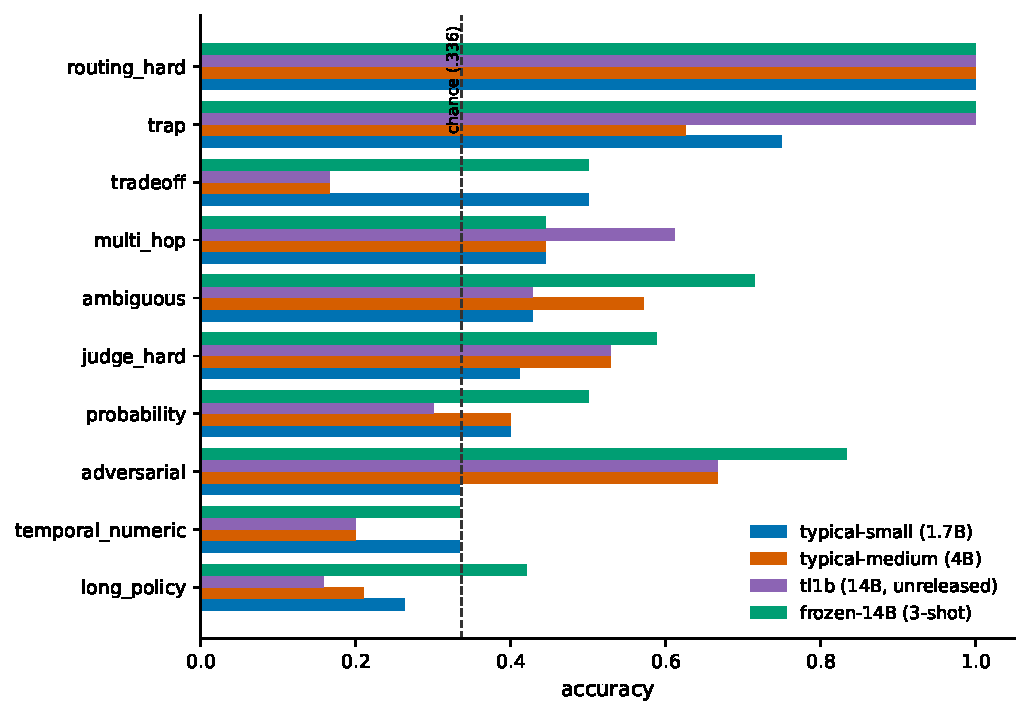
\includegraphics[width=\linewidth]{figures/fig_hard_families.pdf}
  \caption{\textbf{Public subset, unranked.} Per-family JevBench-hard accuracy for the v1 release
  checkpoints (\texttt{ts1b}, \texttt{tm1b}), the 14B checkpoint \texttt{tl1b}, and the frozen-14B
  3-shot control, chance line at .336. Per-family $n$ ranges from 4 to 19 items; no single family
  separates, and the direction across the serial families is uniform. Values are read directly from each
  run's JSON evaluation artifact.}
  \label{fig:hard_families}
\end{figure}

\subsubsection{Per-family JevBench-hard table}
\label{app:hard-families}

\Cref{tab:app-hard} gives the hard-tier sub-families at 14B. The frozen-control column and the
\texttt{ambiguous} row are read from each run's JSON evaluation artifact. For \texttt{ladder\_14b}'s
temporal and probability cells, the JSON artifact and the project's internal report disagree (.333/.50
in the JSON vs.\ .20/.40 in the report); the table gives the report values, marked $\dagger$.

\begin{table}[h]
  \centering
  \caption{JevBench hard-tier sub-family accuracy, 14B. \textbf{Public subset, unranked};
  per-family cells are 3--19 items each and carry no useful interval.}
  \label{tab:app-hard}
  \small
  \begin{tabular}{lrrr}
    \toprule
    Sub-family & \texttt{ladder\_14b} & \texttt{tl1b} & Frozen 14B, 3-shot \\
    \midrule
    long\_policy & .05 & .158 & .421 \\
    multi\_hop & .44 & .611 & .444 \\
    trap & 1.00 & 1.00 & 1.00 \\
    adversarial & .67 & .667 & .833 \\
    ambiguous & .429 & .429 & .714 \\
    temporal & .20\textsuperscript{$\dagger$} & .20 & .333 \\
    probability & .40\textsuperscript{$\dagger$} & .30 & .50 \\
    tradeoff & .67 & .17 & .50 \\
    \bottomrule
  \end{tabular}

  \vspace{2pt}
  \raggedright\footnotesize $\dagger$ The JSON-derived values for these two \texttt{ladder\_14b} cells
  are .333 (temporal) and .50 (probability).
\end{table}

\subsection{Closed-loop decisions: a case study}
\label{app:closed-loop}

We drove three games with \texttt{typical-small} through the public decision API, one decision per tick,
on a laptop (Apple M4 Pro, MPS; the probes ran against the v1 weights, before the v2 upload). Each tick
the game engine renders the current situation as the state, offers the legal actions as the candidate
set, and executes the argmax. The state holds only the situations that currently apply, each written as
a sentence that already contains the comparison a rule needs. Drive and Doom put a precedence-ordered
list of one-condition rules in the question; Snake encodes its rules in the state sentences and asks a
plain question. Accuracy is agreement with the literal rule list applied over the offered actions
(\Cref{tab:app-closed-loop}).

\begin{table}[h]
  \centering
  \caption{Closed-loop decisions with \texttt{typical-small}. ``Probe'' is agreement with the literal
  rule list on scripted situations; ``chance'' is uniform over the offered legal actions; ``no rules''
  keeps the state and replaces the rule list with a goal question.}
  \label{tab:app-closed-loop}
  \small
  \setlength{\tabcolsep}{3pt}
  \begin{tabular}{lp{3.1cm}rrrp{4.2cm}}
    \toprule
    Game & Candidates (legal actions) & Probe & Chance & No rules & Recorded run \\
    \midrule
    Drive & 7 manoeuvres, lane changes only when legal & 70/70 & .16 & .157 & 231/231 ticks match the rules; 18/18 red lights, 3 lane changes, exit taken \\
    Doom (aiming) & retreat, shoot, turn left, turn right, explore; no shoot at 0 ammo & 48/48 & .20 & .729 & arena 240/240, 8 kills; E1M1 200/200 (133 explore, 64 shoot, 3 turn), 4 kills \\
    Snake & safe moves & .984 & .48 & -- & 216/217 ticks, 24 food \\
    \bottomrule
  \end{tabular}
\end{table}

\textbf{Drive.} The rule list is \texttt{stop}, \texttt{brake}, \texttt{change lane right},
\texttt{accelerate}, \texttt{change lane left}, \texttt{follow}, and a \texttt{hold speed} default, with
lane changes removed from the candidate set when the lane is occupied or leads away from the exit. The
model matched the rules on 70 scripted situations, including 14/14 exit lane changes and 15/15
overtakes. Removing the guardrail and offering all seven actions drops agreement to .771.

\textbf{Doom.} The model picks one of five actions and the engine presses the key, with a closed-loop
turn by the enemy's bearing. On 48 scripted situations it matched the rules 48/48, including 29/29
turns, and it matched 20/20 sentences in the real engine's vocabulary. In a recorded run on DOOM's
E1M1, with the engine walking a scripted route when the model chooses \texttt{explore}, all 200
decisions match the rule list: 133 explore, 64 shoot and 3 turns, for 4 kills.

\textbf{Snake.} The state is sentences such as ``The snake must move right to close the larger gap to
the food.'' and ``Moving left hits the snake's body.'', the question is ``Which move brings the snake
closer to the food without dying?'', and the candidates are the safe moves. It matched the literal
greedy policy on 61 of 62 boards (.984). Moving the same rules into the question as four direction
rules without a default scored .82--.95 with $\pnull$ .84--.94.

\textbf{What the rendering controls.} The same weights and the same rules succeed or fail depending on
how the state is written, which makes these games a closed-loop instance of \Cref{sec:results:rendering}.
Four regularities held across games.
\begin{itemize}
  \item \emph{Agent-subject sentences that pre-compute the comparison fire their rule.} ``The player
  must turn left to face the enemy.'' fires \texttt{turn left} 29/29; the object-location form ``The
  nearest enemy is 5 cells to the left.'' fired 0/12 over five phrasings. In Drive, ``The car must take
  the exit on the right in 200 m.'' fires 11/11, and ``The exit on the right is 200 m ahead.'' 0/11. In
  Snake, the pre-computed sentences score .984 against .774 for the coordinate form ``The food is 3 cells
  to the right and 2 cells up.'' on the same 62 boards.
  \item \emph{An explicit default rule beats ``none of the above''.} ``explore: applies when the player
  sees no enemy'' fires 6/6; ``explore: applies when none of the above rules fire'' fires 0/8, with the
  mass going to \texttt{shoot} and \texttt{retreat}.
  \item \emph{Raw numbers the model would have to compare leak into the decision.} With ``The player has
  41 health and 34 ammo.'' in the state, an imp in the crosshair reads \texttt{retreat} .56 /
  \texttt{shoot} .42; without the sentence \texttt{shoot} is .89. Mid-health crosshair situations score
  .500 with the numbers sentence and 1.000 without it, and 66 of 200 decisions in an earlier recorded
  run failed this way. Health and ammo now live on the game display, outside the state.
  \item \emph{One condition per rule, within the trained list length.} A rule containing ``or'' fires
  everywhere (Drive .30 and .61 with a disjunctive rule vs.\ 1.00 without). A rule at position 6 fired
  0/5 under four phrasings and the same rule at position 4 fired 4--5/5, matching the training shape of
  three rules plus a default.
\end{itemize}

\subsection{Development chronology}
\label{app:chronology}

\Cref{sec:analysis,sec:train,sec:results} are organized by claim. The experiments ran in this order:
(1) a candidate-blind decision-state branch (dual-encoder-style $Z(\state,\query)$ with an energy scorer
over cached candidate embeddings), which produced the ladder of \Cref{tab:blind} and was closed by the
shuffled-question control; (2) a candidate-in-suffix decision pass, comparing letter-logit,
candidate-blind semantic, and contextual-candidate readouts, which produced \Cref{tab:n1n3}; (3) the
last-layer tap and rendered abstain-line diagnoses, which merged a planned two-regime (energy + native)
architecture into a single model; (4) the workflow and uncertainty corpora, the mixture sweep, and null
augmentation; (5) the Qwen3 size ladder at 1.7B/4B/8B/14B with frozen controls; (6) the 14B bundle
(facts-first long-state rendering, \texttt{--drop\_truncated}, DecisionMix v2, typed heads,
calibration-shaped checkpoint selection, frozen-teacher KD) and its matched no-KD control; (7) the
Qwen3.5 port; (8) cluster bootstraps, the matched truncation ablation, and the purpose-built held-out
long-state set, which produced the paired tests of \Cref{app:hard-tier} and the $2\times2$ of
\Cref{sec:results:long}; and (9) the v2 releases, \texttt{ts1c} (\texttt{typical-small}) and
\texttt{tm2} (\texttt{typical-medium}), both trained on the facts-first corpus.

The candidate-blind branch was closed on $\dq$. Each student closed 20--55\% of the chance-to-teacher
accuracy gap, and the shuffled-question control showed that none of the closed gap was
question-dependent. Selection on accuracy would have kept that branch.

\subsection{JevBench leaderboard context}
\label{app:leaderboard}

\Cref{tab:app-leaderboard} places our numbers among other entries scored on the same 231 public ids.
Entries differ in protocol and rendering, several have no method paper, and the 146 private judge items
are not included. The public standard tier has $n_{\mathrm{eff}}{=}36$ independent states, and rendering
alone moves a frozen model by 12.5 points (\Cref{sec:results:rendering}), which exceeds most of the
spread in this table (\Cref{sec:setup:jevbench}).

\begin{table}[h]
  \centering
  \caption{Other entries scored on the same public 231 ids, from the harness's own per-item files.
  \textbf{Public subset, unranked}, for all rows including ours. Majority/chance baselines: .311
  standard, .284 easy, .336 hard. 95\% cluster-bootstrap intervals for our own rows are in
  \Cref{tab:headline,tab:tl1b}; differences smaller than $\pm6$--13 points (standard) or $\pm9$ points
  (hard) are not rankings.}
  \label{tab:app-leaderboard}
  \small
  \begin{tabular}{lrrr}
    \toprule
    Entry (backbone) & standard (72) & easy (48) & hard (111) \\
    \midrule
    open-jev-deberta-v3-large (classifier) & .431 & 1.00 & .378 \\
    GLiNER2 & .639 & 1.00 & .369 \\
    jeff (GLiFormer 400M) & .750 & 1.00 & .387 \\
    Laya (ModernBERT) & .694 & 1.00 & .351 \\
    open-alternative-jev (Qwen3.5-4B) & .833 & 1.00 & .568 \\
    system-one-open (Gemma E2B LoRA) & .931 & 1.00 & .486 \\
    SemIf (Qwen3.5-4B) & .986 & 1.00 & .613 \\
    OpenJev (26B-A4B) & .972 & 1.00 & .640 \\
    Jev 1.13.0 (closed) & .986 & 1.00 & .730 \\
    \midrule
    Typical, Qwen3-14B (\texttt{tl1b}) & .931 & 1.00 & .450 \\
    Typical, Qwen3.5-4B (\texttt{tm2}, \texttt{typical-medium} v2) & .861 & 1.00 & .495 \\
    \bottomrule
  \end{tabular}
\end{table}

\subsection{Long-state truncation: distributions and the held-out evaluation set}
\label{app:truncation}

\Cref{fig:truncation} gives the \texttt{data\_wf\_long} state-length histogram with truncation fractions
at 256/1024/2048/3072 tokens, which is the measurement behind the 98.8\% figure of
\Cref{sec:train:long}, together with \texttt{long\_policy} accuracy across the bug/fix sequence. The
tokenizer's \texttt{truncation\_side} is \texttt{'right'}, verified empirically on the released
tokenizer.

The held-out long-state evaluation set (\texttt{scripts/make\_long\_eval.py}, $n{=}605$) was built for
the $2\times2$ of \Cref{tab:twobytwo}. It has zero exact-state overlap with either training corpus, with
\texttt{Case}-stem overlaps dropped, and is scored at a 4{,}096-token window against states with
$p50 = 1{,}965$ and $\max = 2{,}843$ tokens, so no item is truncated at evaluation in any of the eight
cells. The two renderings differ only in whether the evidence block precedes or follows the request
text; the items, labels, and candidate sets are identical. The set shares a generator family with the
training data, and it measures the training defect of \Cref{sec:results:long}. Significance for the
matched-vs-matched comparison is a two-proportion test over the 605 paired items ($z = 6.2$,
$p = 5\times10^{-10}$ at 1.7B; $p = 7\times10^{-12}$ at 14B).

\textbf{Released checkpoints.} The v1 releases were trained before the facts-first fix, and the v2
releases replace them with post-fix checkpoints (\Cref{tab:app-long-release}). On facts-first long
states \texttt{ts1c} gains 34.9 points over \texttt{ts1b} and \texttt{tm2} gains 33.8 over
\texttt{tm1b}, while facts-last accuracy moves by $-0.8$ and $+1.3$. JevBench does not register the
change: \texttt{ts1c} reads .708/.432 against \texttt{ts1b}'s .694/.432.

\begin{table}[h]
  \centering
  \caption{Release checkpoints on the 605 held-out long states (4{,}096-token window, no truncation),
  identical items in both render columns. Majority-class floors: .334 overall, .612 on
  \texttt{policy\_permit}. JevBench is the public 231-id subset, unranked.}
  \label{tab:app-long-release}
  \small
  \setlength{\tabcolsep}{4pt}
  \begin{tabular}{llrrrr}
    \toprule
    Release & Checkpoint & facts-first & facts-last & \texttt{policy\_permit} (first) & JevBench std / hard \\
    \midrule
    \texttt{typical-small} v1 & \texttt{ts1b} & .598 & .798 & .536 & .694 / .432 \\
    \texttt{typical-small} v2 & \texttt{ts1c} & \textbf{.947} & .790 & .948 & .708 / .432 \\
    \texttt{typical-medium} v1 & \texttt{tm1b} & .612 & .866 & .555 & .806 / .423 \\
    \texttt{typical-medium} v2 & \texttt{tm2} & \textbf{.950} & .879 & .967 & .861 / .495 \\
    \bottomrule
  \end{tabular}
\end{table}

\subsection{Operations and reproducibility notes}
\label{app:ops}

Training and evaluation ran on rented RunPod H100 instances (SXM and NVL variants); the infrastructure
issues that affected timing are recorded here for reproducibility. A pod created with an SSH-only startup
flag never reached a ready state on the account used and billed regardless (encountered repeatedly before
being diagnosed); using a fixed exposed port at boot avoided it. Stopping a pod without an attached
persistent volume wipes it, so checkpoints and manifests were always written to a network volume or pushed
to the Hugging Face Hub before a pod was stopped. \texttt{tmux kill-session} does not terminate a
\texttt{timeout}-wrapped child process, which once produced a stray duplicate training run sharing a GPU
with the intended one; process matching over SSH must target the exact command, since a loose
\texttt{pkill} pattern can match and kill the SSH shell itself before the target process. Two pods sharing
one Python environment on the same network volume corrupted it under concurrent dependency resolution;
per-pod environments with dependency syncing disabled avoided this. Every run's manifest records the
harness commit, checkpoint hash, and dependency lock file used, and the JevBench per-item comparisons in
this paper are all computed against the same fixed set of 231 public ids from one harness commit.

\subsection{Full result tables}
\label{app:full-results}

\Cref{tab:app-evidence,tab:app-knowledge,tab:app-wf-eval,tab:app-jevbench,tab:app-latency} give the
complete cross-checkpoint result tables for every checkpoint with a completed evaluation. \texttt{ts1b}
and \texttt{tm1b} are the v1 releases; \texttt{tm2} is \texttt{typical-medium} v2, and \texttt{ts1c}
(\texttt{typical-small} v2) is in \Cref{tab:app-long-release}.

\begin{table}[h]
  \centering
  \caption{Evidence and knowledge-classification accuracy by checkpoint.}
  \label{tab:app-evidence}
  \small
  \setlength{\tabcolsep}{3.5pt}
  \begin{tabular}{llrrrrrrrr}
    \toprule
    Model & Checkpoint & CLINC-150 & TREC-fine & HWU64 & 20NG & SNLI & MNLI & BoolQ & ANLI \\
    \midrule
    Qwen3-1.7B & \texttt{ts1b} & .801 & .508 & .761 & .540 & .894 & .859 & .824 & .497 \\
    Qwen3-4B & \texttt{tm1b} & .847 & .414 & .769 & .588 & .909 & .861 & .843 & .544 \\
    Qwen3-8B & \texttt{ladder\_8b} & .769 & .486 & .740 & .452 & .853 & .831 & .822 & .468 \\
    Qwen3-14B & \texttt{tl1b} & .827 & .508 & .760 & .690 & .911 & .868 & .882 & .583 \\
    Qwen3.5-4B & \texttt{tm2} & .795 & .480 & .717 & .579 & .900 & .855 & .840 & .554 \\
    \bottomrule
  \end{tabular}
\end{table}

\begin{table}[h]
  \centering
  \caption{Knowledge probe (MMLU-Pro among-$K$, $\dqsh$) and TruthfulQA MC1.}
  \label{tab:app-knowledge}
  \small
  \begin{tabular}{llrrr}
    \toprule
    Model & Checkpoint & MMLU-Pro among-$K$ & $\dqsh$ & TruthfulQA MC1 \\
    \midrule
    Qwen3-1.7B & \texttt{ts1b} & .343 & .127 & .257 \\
    Qwen3-4B & \texttt{tm1b} & .458 & .193 & .408 \\
    Qwen3-8B & \texttt{ladder\_8b} & .302 & .093 & .277 \\
    Qwen3-14B & \texttt{tl1b} & .498 & .235 & .481 \\
    Qwen3.5-4B & \texttt{tm2} & .429 & .194 & .414 \\
    \bottomrule
  \end{tabular}
\end{table}

\begin{table}[h]
  \centering
  \caption{Held-out workflow and external floors. Rows marked \emph{full} are the post-hoc
  \texttt{eval\_wf} pass over every row at full state length (4{,}096-token window,
  \texttt{--limit 0}); rows marked \emph{train-time} are the 1{,}500-row, 256-token pass emitted
  during training, which truncates the long external sets and is not comparable to the full pass.
  The distinction is load-bearing on the external sets: on \texttt{ts1b}, PagerDuty reads .560 at
  train time and .817 at full length, because the 256-token window removes the incident text.
  Numbers in parentheses after held-out score are NLL.}
  \label{tab:app-wf-eval}
  \small
  \setlength{\tabcolsep}{2.5pt}
  \begin{tabular}{llrrrrrr}
    \toprule
    Model & Pass & \shortstack{Held-out\\noul} & \shortstack{Held-out\\score (NLL)} & \shortstack{Held-out\\style} & \shortstack{PagerDuty\\(.792)} & \shortstack{jevlogs\\(.697)} & \shortstack{Mind2Web\\(.427)} \\
    \midrule
    \texttt{ts1b} & full & .715 & .520 (1.01) & .859 & \textbf{.817} & \textbf{.710} & .357 \\
    \texttt{tm1b} & full & .811 & .528 (1.03) & .859 & \textbf{.838} & .673 & .544 \\
    \texttt{tl1b} & full & .831 & .623 (0.95) & .880 & \textbf{.878} & .546 & .563 \\
    \midrule
    \texttt{ladder\_8b} & train-time & .681 & .543 (1.72) & .882 & .321 & .501 & .404 \\
    \texttt{tm2} & train-time & .858 & .586 (0.97) & .842 & .757 & .518 & .497 \\
    \bottomrule
  \end{tabular}
\end{table}

\begin{table}[h]
  \centering
  \caption{JevBench accuracy (Brier). \textbf{Public subset, unranked} (72 standard over 36
  paraphrase-clustered states / 48 easy / 111 hard); see \Cref{tab:headline,tab:tl1b} for intervals.}
  \label{tab:app-jevbench}
  \small
  \begin{tabular}{lrrr}
    \toprule
    Model (checkpoint) & Standard (Brier) & Easy (Brier) & Hard (Brier) \\
    \midrule
    Qwen3-1.7B (\texttt{ts1b}) & .694 (.40) & 1.00 (.005) & .432 (.79) \\
    Qwen3-4B (\texttt{tm1b}) & .806 (.30) & 1.00 (.012) & .423 (.77) \\
    Qwen3-8B (\texttt{ladder\_8b}) & .667 (.55) & 1.00 (.015) & .396 (.83) \\
    Qwen3-14B (\texttt{tl1b}) & \textbf{.931} (.18) & 1.00 (.005) & .450 (.66) \\
    Qwen3.5-4B (\texttt{tm2}) & .861 (.22) & 1.00 & \textbf{.495} (.72) \\
    Qwen3.5-4B, frozen 3-shot & .764 (.36) & 1.00 & .495 (.60) \\
    Qwen3.5-9B, frozen semif-render & .931 (.11) & 1.00 & .595 (.51) \\
    Qwen3-14B, frozen 3-shot & .819 (.28) & 1.00 & .559 (.56) \\
    \bottomrule
  \end{tabular}
\end{table}

\begin{table}[h]
  \centering
  \caption{Single-decision latency (same-pod, same-torch-build; ms), $L_s{=}256$.}
  \label{tab:app-latency}
  \small
  \begin{tabular}{lrrrr}
    \toprule
    Model (checkpoint) & $K{=}2$ & $K{=}32$ & $K{=}256$ & Peak memory $K{=}2{\to}256$ (GB) \\
    \midrule
    Qwen3-1.7B (\texttt{ts1b}-shape) & 45 & 46 & 106 & 6.4 $\to$ 9.3 \\
    Qwen3-4B (\texttt{tm1b}) & 57 & 58 & 96 & 14.6 $\to$ 18.6 \\
    Qwen3-8B (\texttt{ladder\_8b}) & 70 & 71 & 126 & 29.3 $\to$ 34.1 \\
    Qwen3-14B (\texttt{tl1b}) & 59 & 62 & 156 & 51.6 $\to$ 57.5 \\
    \bottomrule
  \end{tabular}
\end{table}
